\section{Инфологическая модель локальной телекоммуникационной системы организации}
\label{sec:inf_model}
В ходе выполнения задания требовалось определить бизнес-цель организациии. Бизнес-целью торгового склада является предоставление потребителям необходимых строительных материалов.

Для достижения этой цели торговый склад выполняет следующие функции:
\begin{itemize}
\item прием товара от поставщиков;
\item учет товара;
\item выдачу товара покупателям;
\item подготовление отчетности;
\item передача информации продавцу наличии/отсутствии товара.
\end{itemize}


Для ТКС торгового склада целевой функцией может являться автоматизация учета товара. ТКС может быть задействована в следующих процессах:
\begin{itemize}
\item контроль операций с товаром;
\item установление кантакта с поставщиками;
\item предоставление доступа к сайту/БД;
\item печать документов;
\item составление и отправка отчетности в контроллирующие органы.
\end{itemize}


Была проведена декомпозиция целевой функции системы для детального описания процессов, необходимых для ее выполнения. Описание процессов проведено с помощью методологии функционального моделирования IDEF0. Результат выполнения декомпозиции приведен на рисунках \ref{fig:idef0-common} и \ref{fig:idef0-inside}.

\begin{sidewaysfigure}[!htp]
  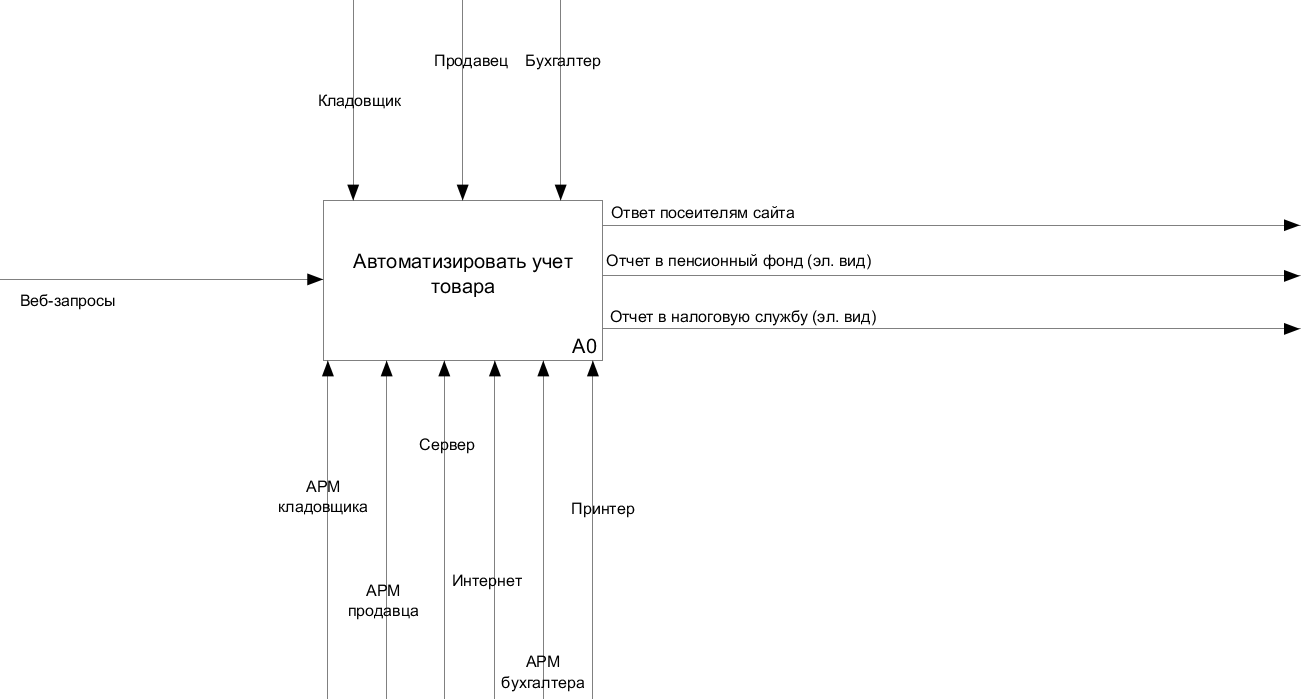
\includegraphics[width=\linewidth]{appendix/a0.png}
  \caption{Целевая функция телекоммуникационной системы торгового склада}
  \label{fig:idef0-common}
\end{sidewaysfigure}
\clearpage

\begin{sidewaysfigure}[!htp]
  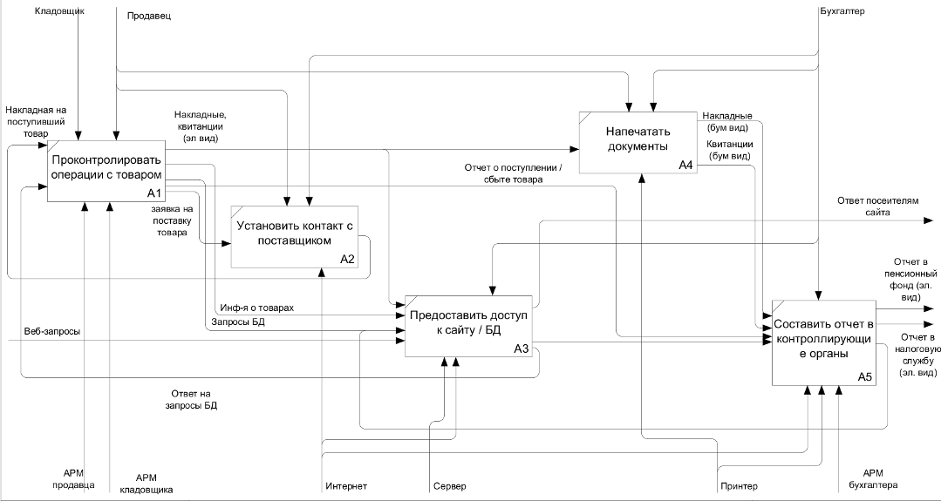
\includegraphics[width=\linewidth]{appendix/a0_2.png}
  \caption{Декомпозиция целевой функции ТКС торгового склада}
  \label{fig:idef0-inside}
\end{sidewaysfigure}
\clearpage

Графическое представление процессов приведено на рисунках \ref{fig:a1}, \ref{fig:a2}, \ref{fig:a3}, \ref{fig:a4}, \ref{fig:a5}.

\begin{figure}[H]
  \centering
  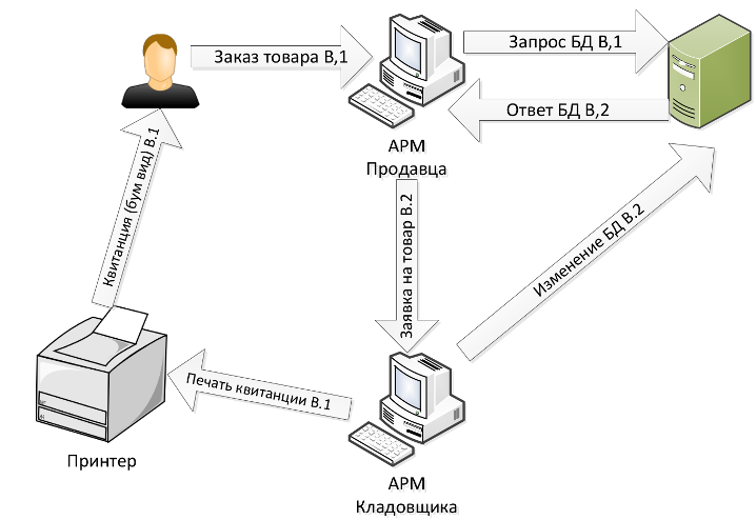
\includegraphics[width=\linewidth]{sec1/img/a1.png}
  \caption{Процесс контроля операций с товаром}
  \label{fig:a1}
\end{figure}

\begin{figure}[H]
  \centering
  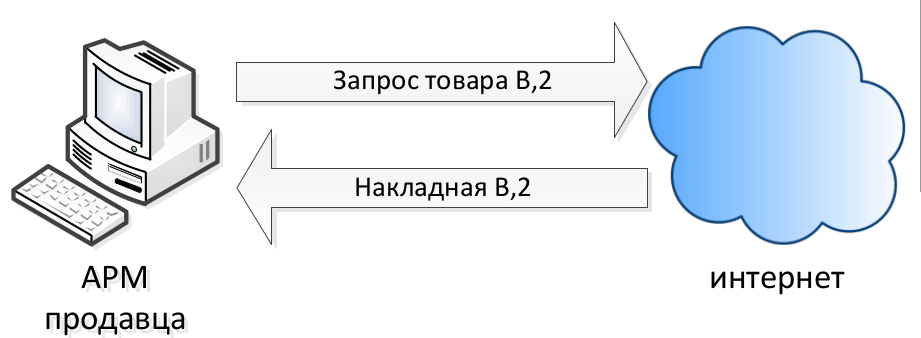
\includegraphics[width=\linewidth]{sec1/img/a2.png}
  \caption{Процесс установки контакта с поставщиком}
  \label{fig:a2}
\end{figure}

\begin{figure}[H]
  \centering
  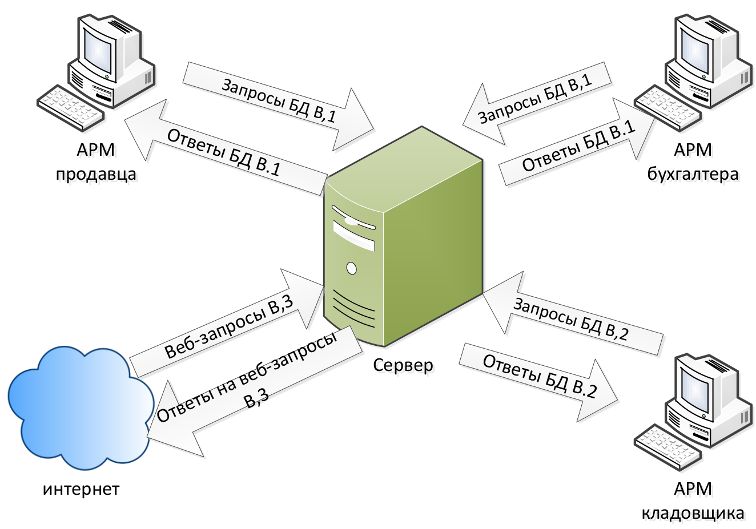
\includegraphics[width=\linewidth]{sec1/img/a3.png}
  \caption{Процесс предоставления доступа к сайту/БД}
  \label{fig:a3}
\end{figure}


\begin{figure}[H]
  \centering
  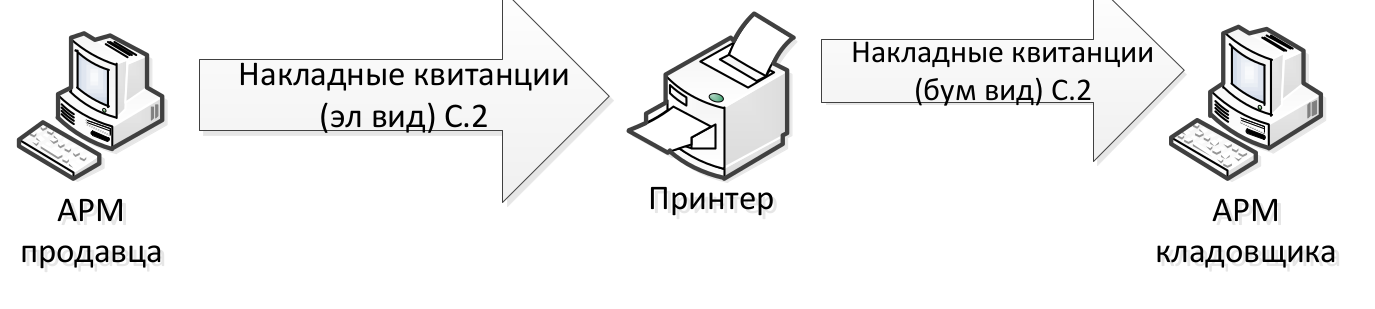
\includegraphics[width=\linewidth]{sec1/img/a4.png}
  \caption{Процесс печати документов}
  \label{fig:a4}
\end{figure}

\begin{figure}[H]
  \centering
  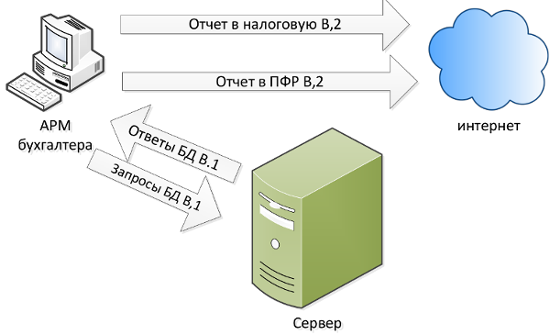
\includegraphics[width=\linewidth]{sec1/img/a5.png}
  \caption{Процесс составления и отправки отчетности}
  \label{fig:a5}
\end{figure}

Общая инфологическая модель телекоммуникационной системы торгового склада приведена на рисунке \ref{fig:total}.

\begin{figure}[H]
  \centering
  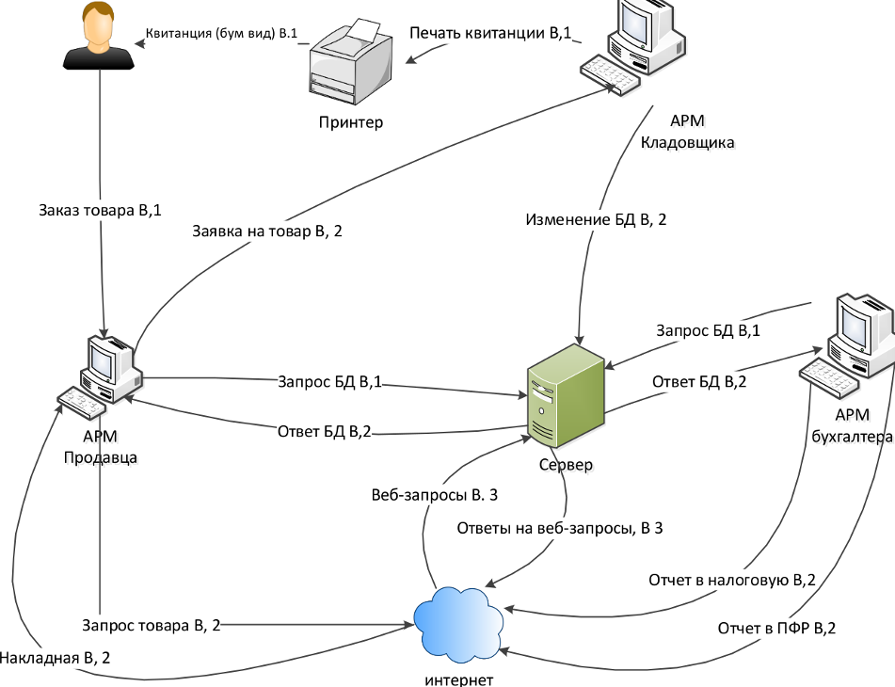
\includegraphics[width=\linewidth]{sec1/img/total.png}
  \caption{Общая инфологическая модель телекоммуникационной системы торгового склада}
  \label{fig:total}
\end{figure}

